% Sprawozdanie z badań metaheurystyk dla PFSP
\documentclass[11pt,a4paper]{article}
\usepackage[margin=1in]{geometry}
\usepackage[utf8]{inputenc}
\usepackage{polski}
\usepackage{graphicx}
\usepackage{booktabs}
\usepackage{array}
\usepackage{longtable}
\usepackage{float}
\usepackage{caption}
\usepackage{hyperref}
\usepackage{pdflscape}

\title{Metody Optymalizacji\\Projekt: PFSP}
\author{Jakub Wasilewski 263852}
\date{10.04.2026}

\begin{document}
\maketitle

\tableofcontents
\clearpage

\section{Sformułowanie zadania}
Celem zadania była implementacja i przebadanie metaheurystyki Algorytmu Ewolucyjnego (EA) dla permutacyjnego problemu przepływowego (PFSP -- \textit{Permutation Flow Shop Problem}) oraz porównanie jej z metodami nieewolucyjnymi: algorytmem zachłannym (greedy), symulowanym wyżarzaniem (SA) i losowym przeszukiwaniem.

W PFSP rozpatrywano $n$ zadań i $m$ maszyn. Każde zadanie musiało być wykonane na każdej maszynie w tej samej ustalonej kolejności (maszyna 1 $\rightarrow$ 2 $\rightarrow \ldots \rightarrow$ m). Czas przetwarzania zadania $j$ na maszynie $i$ wynosił $p_{ij}$. Poszukiwano permutacji zadań minimalizującej \textbf{makespan} -- czas zakończenia ostatniego zadania na ostatniej maszynie ($C_{\max}$).

\section{Sposób rozwiązywania zadania}
Rozwiązania były kodowane jako permutacje $n$ zadań. Ocena rozwiązania polegała na obliczeniu makespanu poprzez symulację harmonogramu: dla każdej maszyny i każdego zadania (w kolejności permutacji) czas zakończenia wyznaczany był jako maksimum czasu zwolnienia maszyny i czasu zakończenia poprzedniego zadania na tej samej maszynie, powiększony o czas przetwarzania. Wszystkie metaheurystyki operowały bezpośrednio na permutacjach.

\section{Metody użyte do rozwiązania zadania}
\begin{itemize}
  \item Algorytm losowy (random)
  \item Algorytm zachłanny (greedy, multi-start)
  \item Symulowane wyżarzanie (SA)
  \item Algorytm ewolucyjny (EA)
\end{itemize}

\section{Implementacja}

\subsection{Algorytm losowy}
\label{sec:random}
\begin{itemize}
    \item Zastosowano proste losowe przeszukiwanie przestrzeni rozwiązań.
    \item W każdej iteracji generowana była losowa permutacja $n$ zadań i obliczany jej makespan.
    \item \textbf{Parametry:} liczba iteracji = budżet $B$.
    \item \textbf{Log:} co iterację zapisywany był bieżący koszt; Logger śledził best/avg/worst w czasie.
\end{itemize}

\subsection{Algorytm zachłanny}
\label{sec:greedy}
\begin{itemize}
    \item Zaimplementowano wielostartowy algorytm konstrukcyjny.
    \item Dla każdego punktu startowego (zadania) budowana była permutacja -- w każdym kroku kolejne zadanie wstawiano na pozycję minimalizującą bieżący makespan (podejście NEH-like).
    \item \textbf{Multi-start:} przeprowadzano uruchomienia dla różnych zadań startowych; zwracane było najlepsze znalezione rozwiązanie.
    \item \textbf{Parametry:} liczba restartów (domyślnie = liczba zadań).
\end{itemize}

\subsection{Symulowane wyżarzanie (SA)}
\label{sec:sa}
\begin{itemize}
    \item Zaimplementowano metaheurystykę inspirowaną procesem wyżarzania metali.
    \item \textbf{Rozwiązanie startowe:} losowa permutacja (nowe w każdym uruchomieniu).
    \item \textbf{Sąsiedztwo:} operator swap -- zamiana dwóch losowych pozycji w permutacji.
    \item \textbf{Akceptacja:}
    \begin{itemize}
        \item Ruch poprawiający ($\Delta < 0$): zawsze był akceptowany.
        \item Ruch pogarszający: akceptowany z prawdopodobieństwem $\exp(-\Delta/T)$.
    \end{itemize}
    \item \textbf{Schemat chłodzenia:} geometryczny, $T_{t+1} = \alpha \cdot T_t$, gdzie $\alpha$ to współczynnik chłodzenia.
    \item \textbf{Temperatura początkowa $T_0$:} estymowana była automatycznie ze wzoru
    $T_0 = -\overline{\Delta^+} / \ln(p_0)$,
    gdzie $\overline{\Delta^+}$ to średni dodatni delta z 200 losowych ruchów swap, a $p_0 = 0{,}8$ to docelowe prawdopodobieństwo akceptacji ruchu pogarszającego na starcie.
    \item \textbf{Kryterium stopu:} po wykonaniu dokładnie $B$ ewaluacji (kroków pętli).
\end{itemize}

\subsection{Algorytm ewolucyjny (EA)}
\label{sec:ea}
\begin{itemize}
    \item Zaimplementowano metaheurystykę inspirowaną ewolucją biologiczną.
    \item \textbf{Inicjalizacja:} tworzona była populacja losowych permutacji (rozmiar \texttt{pop\_size}), każda oceniana -- koszt $= 1$ ewaluacja.
    \item \textbf{Selekcja:} turniejowa -- losowano \texttt{tour\_size} osobników i wybierano najlepszego.
    \item \textbf{Krzyżowanie:}
    \begin{itemize}
        \item \textbf{OX} (Ordered Crossover) -- kopiowany był segment z rodzica 1, brakujące elementy uzupełniano w kolejności z rodzica 2, zachowując względną kolejność.
        \item \textbf{PMX} (Partially Mapped Crossover) -- wymieniano segmenty i naprawiano konflikty przez mapowanie pozycji.
        \item \textbf{CX} (Cycle Crossover) -- zachowywane były bezwzględne pozycje genów przez cykl mapowania.
        \item Krzyżowanie stosowane było z prawdopodobieństwem \texttt{Px}; w przeciwnym razie kopiowany był rodzic 1.
    \end{itemize}
    \item \textbf{Mutacja:}
    \begin{itemize}
        \item \textbf{SWAP} -- zamiana dwóch losowych pozycji w permutacji.
        \item \textbf{INVERSION} -- odwrócenie losowego segmentu permutacji.
        \item Mutacja stosowana była z prawdopodobieństwem \texttt{Pm}.
    \end{itemize}
    \item \textbf{Kryterium stopu:} po wykonaniu dokładnie $B$ ewaluacji.
    \item \textbf{Budżet:} $\texttt{pop\_size} \cdot (\texttt{gen} + 1) = B$, gdzie $+1$ uwzględnia koszt inicjalizacji populacji. Stąd $\texttt{gen} = (B - \texttt{pop\_size}) / \texttt{pop\_size}$.
\end{itemize}

\subsection{Kontrola budżetu}
Wszystkie algorytmy korzystały ze wspólnego licznika wywołań funkcji celu (\texttt{eval\_counter}) w klasie \texttt{PfspInstance}. Po każdym eksperymencie weryfikowany był assert: dla EA -- $N\_RUNS \cdot B$, dla SA -- $N\_RUNS \cdot (B+1)$ (dodatkowe wywołanie z losowego startu).

\section{Pliki wejściowe}
Wykorzystano instancje z zestawu benchmarkowego Taillarda:
\begin{itemize}
    \item \textbf{Łatwe:} tai20\_5 (20 zadań, 5 maszyn), tai20\_10 (20 zadań, 10 maszyn), tai20\_20 (20 zadań, 20 maszyn)
    \item \textbf{Średnie:} tai100\_10 (100 zadań, 10 maszyn), tai100\_20 (100 zadań, 20 maszyn)
    \item \textbf{Trudne:} tai500\_20 (500 zadań, 20 maszyn)
\end{itemize}

\section{Procedura badawcza}
\begin{itemize}
    \item Budżet obliczeniowy: $B = 100\,000$ wywołań funkcji celu dla wszystkich konfiguracji.
    \item Liczba powtórzeń: $N = 5$ niezależnych uruchomień.
    \item Miara jakości: \textbf{średnia} (avg) wyników z $N$ powtórzeń -- odporna na pojedyncze szczęśliwe wyniki.
    \item Parametry bazowe EA: \texttt{pop\_size=100}, \texttt{Px=0.7}, \texttt{Pm=0.1}, \texttt{tour\_size=5}, krzyżowanie OX, mutacja SWAP, inicjalizacja losowa.
    \item Parametry bazowe SA: $T_0$ auto-estymowane, $\alpha=0{,}995$.
\end{itemize}

\section{Wyniki badań przed strojeniem}
\label{sec:baseline}

Poniższa tabela przedstawia wyniki uzyskane z domyślnymi parametrami ($N=5$ powtórzeń, $B=100\,000$). Dla EA zastosowano: \texttt{pop=100}, \texttt{gen=999}.

\begin{table}[H]
\centering
\caption{Wyniki bazowe (przed strojeniem)}
\begin{tabular}{lrrrrrrrr}
\toprule
Instancja & EA best & EA avg & EA std & SA best & SA avg & SA std \\
\midrule
tai20\_5   & 14094 & 14190 & 75.7  & 14163 & 14359 & 196.2 \\
tai20\_10  & 21432 & 21692 & 257.2 & 21001 & 21547 & 436.8 \\
tai20\_20  & 33972 & 34451 & 268.6 & 34320 & 34422 & 60.0  \\
tai100\_10 & 314007 & 317724 & 2968.3 & 309957 & 311563 & 1634.6 \\
tai100\_20 & 386480 & 389944 & 2594.4 & 385105 & 386373 & 1391.6 \\
tai500\_20 & 7218198 & 7238642 & 13201.4 & 6998539 & 7027898 & 17267.2 \\
\bottomrule
\end{tabular}
\end{table}

\textbf{Wnioski (etap bazowy):}
\begin{itemize}
    \item Na małych instancjach (tai20\_*) EA z domyślną populacją 100 okazał się konkurencyjny lub lepszy od SA.
    \item Na dużych instancjach (tai100\_*, tai500\_20) SA wyraźnie dominowało -- przewaga rosła ze skalą problemu (dla tai500\_20 SA było lepsze o ok. 3\%).
    \item Duże odchylenie standardowe EA wskazywało na niestabilność przy małej populacji.
\end{itemize}

\section{Strojenie parametrów}
\label{sec:tuning}

Strojenie przeprowadzono iteracyjnie, każdorazowo utrwalając najlepszy parametr przed przejściem do kolejnego. Budżet $B = 100\,000$ dla wszystkich konfiguracji.

\subsection{Rozmiar populacji (\texttt{pop\_size})}

Przetestowano wartości: 100, 200, 500, 1000, 5000, 10000. Liczba generacji dobierana była automatycznie: $\texttt{gen} = (B - \texttt{pop}) / \texttt{pop}$.

\begin{table}[H]
\centering
\caption{Strojenie \texttt{pop\_size} -- avg z 5 uruchomień}
\begin{tabular}{lrrrrrr}
\toprule
pop\_size (gen) & tai20\_5 & tai20\_10 & tai20\_20 & tai100\_10 & tai100\_20 & tai500\_20 \\
\midrule
100 (999)    & 14190 & 21692 & 34451 & 317724 & 389944 & \textbf{7238642} \\
200 (499)    & 14250 & 21232 & 34118 & 315830 & 389927 & 7263246 \\
500 (199)    & 14119 & 21091 & 33956 & 315084 & 389878 & 7289871 \\
1000 (99)    & 14083 & 20997 & 33947 & 314121 & 390081 & 7298239 \\
5000 (19)    & \textbf{14054} & \textbf{20975} & \textbf{33837} & 331266 & 407276 & 7623762 \\
10000 (9)    & 14296 & 21489 & 34371 & 341050 & 419076 & 7738554 \\
\bottomrule
\end{tabular}
\end{table}

\textbf{Wnioski:} Ujawniła się odwrotna zależność między optymalnym \texttt{pop\_size} a trudnością instancji. Na małych instancjach duża populacja (5000) wygrywała -- przestrzeń rozwiązań była mała, a różnorodność genetyczna okazała się ważniejsza niż liczba generacji. Na dużych instancjach mała populacja z wieloma generacjami (100, 999 gen) wygrywała -- przestrzeń była ogromna, algorytm potrzebował głębokiej iteracyjnej poprawy, a nie szerokiej inicjalizacji. Przy \texttt{pop=5000} na tai100/tai500 liczba generacji spadała do 9--19, co praktycznie uniemożliwiało ewolucję.

\textbf{Przyjęte wartości:} \texttt{pop=5000} dla instancji tai20\_*, \texttt{pop=500} dla tai100\_* i tai500\_20.

\subsection{Operatory genetyczne}

Przetestowano macierz 3 operatorów krzyżowania × 2 operatorów mutacji = 6 kombinacji, przy domyślnych \texttt{Px=0.7}, \texttt{Pm=0.1}.

\begin{table}[H]
\centering
\caption{Strojenie operatorów -- avg z 5 uruchomień}
\begin{tabular}{lrrrrrr}
\toprule
Operatory & tai20\_5 & tai20\_10 & tai20\_20 & tai100\_10 & tai100\_20 & tai500\_20 \\
\midrule
\textbf{OX+SWAP}  & \textbf{14050} & \textbf{20976} & \textbf{33804} & \textbf{314976} & \textbf{388839} & \textbf{7269054} \\
OX+INV   & 14050 & 20985 & 33839 & 320988 & 394008 & 7396331 \\
PMX+SWAP & 14096 & 21155 & 34012 & 316063 & 390552 & 7295316 \\
PMX+INV  & 14114 & 21122 & 34031 & 323640 & 399469 & 7475300 \\
CX+SWAP  & 14251 & 21392 & 34253 & 318466 & 392366 & 7373814 \\
CX+INV   & 14200 & 21432 & 34289 & 326987 & 405567 & 7536259 \\
\bottomrule
\end{tabular}
\end{table}

\textbf{Wnioski:} Kombinacja OX+SWAP wygrała we wszystkich sześciu instancjach.

SWAP okazał się lepszy od INVERSION niezależnie od krzyżowania -- w PFSP kluczowa jest \emph{względna kolejność} zadań, a nie bezwzględne pozycje. INVERSION odwracał segment, niszcząc starannie wypracowane przez OX bloki kolejności. SWAP zamieniał tylko dwa elementy, zachowując resztę struktury.

CX wypadł najgorzej -- jest zaprojektowany do zachowania bezwzględnych pozycji genów, co nie ma znaczenia w PFSP.

PMX uplasował się pośrodku -- częściowe mapowanie dawało lepsze wyniki niż CX, ale gorsze niż OX. OX najlepiej zachowywał ciągłe bloki względnej kolejności, co odpowiadało strukturze dobrego harmonogramu w PFSP.

\textbf{Przyjęta konfiguracja:} \texttt{crossover = OX}, \texttt{mutation = SWAP}.

\subsection{Prawdopodobieństwo krzyżowania (\texttt{Px})}

Przetestowano wartości: 0.50, 0.70, 0.90, 0.95, 0.98. Zastosowano operatory OX+SWAP oraz per-instancja \texttt{pop\_size}.

\begin{table}[H]
\centering
\caption{Strojenie \texttt{Px} -- avg z 5 uruchomień}
\begin{tabular}{lrrrrrr}
\toprule
Px & tai20\_5 & tai20\_10 & tai20\_20 & tai100\_10 & tai100\_20 & tai500\_20 \\
\midrule
0.50 & 14067 & 20977 & 33858 & 318557 & 391250 & 7318585 \\
0.70 & 14049 & 20978 & \textbf{33769} & 316222 & 390330 & 7273954 \\
0.90 & \textbf{14045} & \textbf{20947} & 33773 & \textbf{311625} & 387485 & 7205858 \\
0.95 & 14058 & 20964 & 33803 & 313028 & \textbf{384112} & 7206759 \\
0.98 & 14049 & 20963 & 33831 & 311889 & 385569 & \textbf{7185858} \\
\bottomrule
\end{tabular}
\end{table}

\textbf{Wnioski:} Im trudniejsza instancja, tym wyższe \texttt{Px} okazywało się korzystniejsze. Na małych instancjach różnice były marginalne (szum przy $N=5$). Na dużych instancjach wzrost \texttt{Px} od 0.50 do 0.98 dał wyraźną poprawę (tai500\_20: $-1{,}8\%$).

Krzyżowanie jest operatorem budowania rozwiązań z fragmentów rodziców. W dużej przestrzeni dobre częściowe struktury były rzadkie -- krzyżowanie pozwalało je łączyć. Przy niskim \texttt{Px} EA degenerował się do lokalnego przeszukiwania z mutacją.

\textbf{Przyjęte wartości per-instancja:} tai20\_5: 0.90, tai20\_10: 0.90, tai20\_20: 0.70, tai100\_10: 0.90, tai100\_20: 0.95, tai500\_20: 0.98.

\subsection{Prawdopodobieństwo mutacji (\texttt{Pm})}

Przetestowano wartości: 0.01, 0.05, 0.10, 0.20, 0.40. Zastosowano konfigurację: OX+SWAP, per-instancja \texttt{pop\_size} i \texttt{Px}.

\begin{table}[H]
\centering
\caption{Strojenie \texttt{Pm} -- avg z 5 uruchomień}
\begin{tabular}{lrrrrrr}
\toprule
Pm & tai20\_5 & tai20\_10 & tai20\_20 & tai100\_10 & tai100\_20 & tai500\_20 \\
\midrule
0.01 & \textbf{14046} & 20968 & 33812 & 317763 & 388332 & 7218867 \\
0.05 & 14047 & \textbf{20947} & \textbf{33782} & 314825 & 387514 & 7207249 \\
0.10 & 14062 & 20962 & 33783 & 313286 & 385259 & 7189132 \\
0.20 & 14074 & 20999 & 33818 & 311163 & 383801 & 7180216 \\
0.40 & 14088 & 21049 & 33862 & \textbf{310342} & \textbf{383251} & \textbf{7168178} \\
\bottomrule
\end{tabular}
\end{table}

\textbf{Wnioski:} Zaobserwowano odwrotny wzorzec niż przy \texttt{Px}: im trudniejsza instancja, tym wyższe \texttt{Pm} okazywało się korzystniejsze. Na tai100/tai500 trend był monotonicznie rosnący -- \texttt{Pm=0.40} wygrało wyraźnie (tai500\_20: poprawa o 0.7\% vs \texttt{Pm=0.01}).

Przy dużej przestrzeni i wysokim \texttt{Px} krzyżowanie dominowało reprodukcję -- populacja szybko traciła różnorodność i zbiegała do lokalnego minimum. Mutacja przy wysokim \texttt{Pm} pełniła rolę dywersyfikatora, regularnie wstrzykując perturbacje. Było to szczególnie istotne gdy przestrzeń była wielowymiarowa i pełna lokalnych minimów. \texttt{Px} i \texttt{Pm} działały komplementarnie -- na trudnych instancjach oba parametry powinny być wysokie.

\textbf{Przyjęte wartości per-instancja:} tai20\_5: 0.01, tai20\_10: 0.05, tai20\_20: 0.05, tai100\_10: 0.40, tai100\_20: 0.40, tai500\_20: 0.40.

\subsection{Strojenie parametrów SA}

Przetestowano macierz kombinacji dwóch parametrów:
\begin{itemize}
    \item \textbf{Współczynnik chłodzenia} $\alpha \in \{0.990, 0.995, 0.999\}$
    \item \textbf{Mnożnik temperatury początkowej} $\in \{0.5\times, 1\times, 5\times, 10\times\}$ auto-estymaty ($T_0 = -\overline{\Delta^+}/\ln(0.8)$)
\end{itemize}

Łącznie 12 kombinacji per instancja, $N=5$ powtórzeń, $B=100\,000$.

\begin{table}[H]
\centering
\caption{Strojenie SA -- avg z 5 uruchomień (wybrane wyniki)}
\resizebox{\textwidth}{!}{%
\begin{tabular}{llrrrrrr}
\toprule
$\alpha$ & t0 mult & tai20\_5 & tai20\_10 & tai20\_20 & tai100\_10 & tai100\_20 & tai500\_20 \\
\midrule
0.990 & 0.5$\times$ & 14423 & 21812 & 34490 & 312317 & 387086 & \textbf{6997211} \\
0.990 & 1$\times$   & 14251 & 21741 & 34415 & 313499 & 385459 & 7027637 \\
0.990 & 5$\times$   & 14316 & 22033 & 34506 & 312030 & 385404 & 7011055 \\
0.990 & 10$\times$  & 14262 & 21790 & 34714 & 312374 & 386978 & 7017959 \\
\midrule
0.995 & 0.5$\times$ & 14277 & 21609 & 34383 & 313206 & 385331 & 7027496 \\
0.995 & 1$\times$   & 14334 & 21588 & 34611 & 313006 & 385238 & 7024425 \\
0.995 & 5$\times$   & 14290 & 21707 & 34554 & 313482 & 385612 & 7035818 \\
0.995 & 10$\times$  & 14278 & 21700 & 34447 & 313060 & 387038 & 7005802 \\
\midrule
0.999 & 0.5$\times$ & 14279 & 21585 & 34249 & 313113 & 383319 & 7002763 \\
0.999 & 1$\times$   & 14197 & 21588 & \textbf{34213} & \textbf{310930} & 385280 & 7019722 \\
0.999 & 5$\times$   & 14205 & 21452 & 34452 & 311430 & \textbf{382694} & 7013917 \\
0.999 & 10$\times$  & \textbf{14129} & \textbf{21291} & 34290 & 311087 & 385608 & 7008148 \\
\bottomrule
\end{tabular}}
\end{table}

\subsubsection{Wnioski}

\textbf{Współczynnik chłodzenia:} $\alpha = 0.999$ wygrał na 5 z 6 instancji. Wolne chłodzenie pozwalało algorytmowi spędzić więcej czasu w fazie eksploracji przy umiarkowanej temperaturze -- kluczowe gdy przestrzeń rozwiązań była złożona. Wyjątek stanowiła tai500\_20, gdzie $\alpha = 0.990$ okazał się najlepszy, jednak różnice między wszystkimi konfiguracjami na tej instancji wyniosły poniżej 0.2\% i mieściły się w szumie statystycznym przy $N=5$.

\textbf{Mnożnik $T_0$:} nie zaobserwowano jednoznacznego trendu -- optymalna wartość zależała od instancji. Na małych instancjach (tai20\_5, tai20\_10) wyższe wartości ($10\times$) dawały lepsze wyniki: przy wolnym chłodzeniu wysoka $T_0$ zapewniała długą fazę eksploracji, a mała przestrzeń pozwalała ją w pełni wykorzystać. Na dużych instancjach (tai100\_10, tai100\_20) optymalne okazały się wartości $1\times$--$5\times$, zaś na tai500\_20 niska wartość ($0.5\times$) z szybszym chłodzeniem działała najlepiej -- zbyt wysoka $T_0$ oznaczała trwonienie budżetu na niemal losowe akceptacje zanim algorytm wszedł w fazę eksploatacji.

\textbf{Przyjęte wartości per-instancja:}
\begin{table}[H]
\centering
\begin{tabular}{lcc}
\toprule
Instancja & $\alpha$ & $T_0$ mult \\
\midrule
tai20\_5   & 0.999 & 10$\times$ \\
tai20\_10  & 0.999 & 10$\times$ \\
tai20\_20  & 0.999 & 1$\times$  \\
tai100\_10 & 0.999 & 1$\times$  \\
tai100\_20 & 0.999 & 5$\times$  \\
tai500\_20 & 0.990 & 0.5$\times$ \\
\bottomrule
\end{tabular}
\end{table}

\subsection{Podsumowanie strojeń EA}

\begin{table}[H]
\centering
\caption{Zestawienie finalnych parametrów per instancja}
\begin{tabular}{lcccccccc}
\toprule
 & \multicolumn{5}{c}{EA} & \multicolumn{2}{c}{SA} \\
\cmidrule(lr){2-6} \cmidrule(lr){7-8}
Instancja & \texttt{pop} & \texttt{gen} & \texttt{Px} & \texttt{Pm} & Operatory & $\alpha$ & $T_0$ mult \\
\midrule
tai20\_5   & 5000 & 19  & 0.90 & 0.01 & OX+SWAP & 0.999 & 10$\times$ \\
tai20\_10  & 5000 & 19  & 0.90 & 0.05 & OX+SWAP & 0.999 & 10$\times$ \\
tai20\_20  & 5000 & 19  & 0.70 & 0.05 & OX+SWAP & 0.999 & 1$\times$  \\
tai100\_10 & 500  & 199 & 0.90 & 0.40 & OX+SWAP & 0.999 & 1$\times$  \\
tai100\_20 & 500  & 199 & 0.95 & 0.40 & OX+SWAP & 0.999 & 5$\times$  \\
tai500\_20 & 500  & 199 & 0.98 & 0.40 & OX+SWAP & 0.990 & 0.5$\times$ \\
\bottomrule
\end{tabular}
\end{table}

\textbf{Kluczowe obserwacje:}
\begin{enumerate}
    \item Najważniejszym parametrem okazał się \texttt{pop\_size} -- wpływ na wyniki był największy i jakościowo różny dla małych vs dużych instancji.
    \item Operatory OX+SWAP zdominowały wszystkie instancje. INVERSION i CX nie wniosły korzyści dla PFSP.
    \item \texttt{Px} i \texttt{Pm} wykazały lustrzany wzorzec: na trudnych instancjach oba powinny być wysokie. Krzyżowanie eksplorowało przez rekombinację, mutacja utrzymywała różnorodność.
    \item SA konsekwentnie wygrywało z EA na dużych instancjach, niezależnie od konfiguracji EA. Różnica na tai500\_20 wynosiła ok. 2--3\% na korzyść SA.
\end{enumerate}

\clearpage
\section{Finalne porównanie algorytmów}
\label{sec:final}

Porównanie przeprowadzono z najlepszymi konfiguracjami znalezionymi w etapie strojenia. Parametry dla każdej metody zestawiono w tabeli w sekcji~\ref{sec:tuning}. Zastosowano budżet obliczeniowy $B = 200\,000$ wywołań funkcji celu. Metody niedeterministyczne (Random, EA, SA) uruchomiono $N = 10$ razy niezależnie; wyniki greedy były deterministyczne (jeden przebieg multi-start). Przetestowano wszystkie instancje zestawu Taillarda.

\begin{table}[H]
\centering
\caption{Finalne porównanie -- wyniki z 10 uruchomień ($B = 200\,000$)}
\resizebox{\textwidth}{!}{%
\begin{tabular}{lrrrrrrrrrr}
\toprule
 & \multicolumn{2}{c}{Random} & \multicolumn{1}{c}{Greedy} & \multicolumn{3}{c}{EA} & \multicolumn{3}{c}{SA} \\
\cmidrule(lr){2-3} \cmidrule(lr){4-4} \cmidrule(lr){5-7} \cmidrule(lr){8-10}
Instancja & best & avg & best & best & avg & std & best & avg & std \\
\midrule
tai20\_5   & 14875 & 15038.3 & 15403 & \textbf{14041} & \textbf{14042.9} & 5.7   & 14104 & 14261.3 & 102.6 \\
tai20\_10  & 21999 & 22563.6 & 24611 & \textbf{20911} & \textbf{20952.9} & 15.2  & 21186 & 21360.6 & 121.5 \\
tai20\_20  & 35323 & 35601.2 & 35103 & \textbf{33623} & \textbf{33764.0} & 74.3  & 33972 & 34236.9 & 164.3 \\
tai100\_10 & 355783 & 357195.5 & 373462 & \textbf{307448} & \textbf{309690.9} & 1329.3 & 309629 & 311767.5 & 1369.3 \\
tai100\_20 & 430692 & 433701.8 & 440486 & \textbf{377492} & \textbf{382019.0} & 2431.3 & 381329 & 385474.7 & 2729.2 \\
tai500\_20 & 7840996 & 7879792.0 & 8407645 & 7040703 & 7075627.6 & 34421.2 & -- & -- & -- \\
\bottomrule
\end{tabular}}
\end{table}

\subsection{Wykresy przebiegu EA}

Poniżej przedstawiono przebiegi najlepszego uruchomienia algorytmu ewolucyjnego (best, avg, worst populacji w każdej generacji) dla trzech wybranych instancji.

\begin{figure}[H]
    \centering
    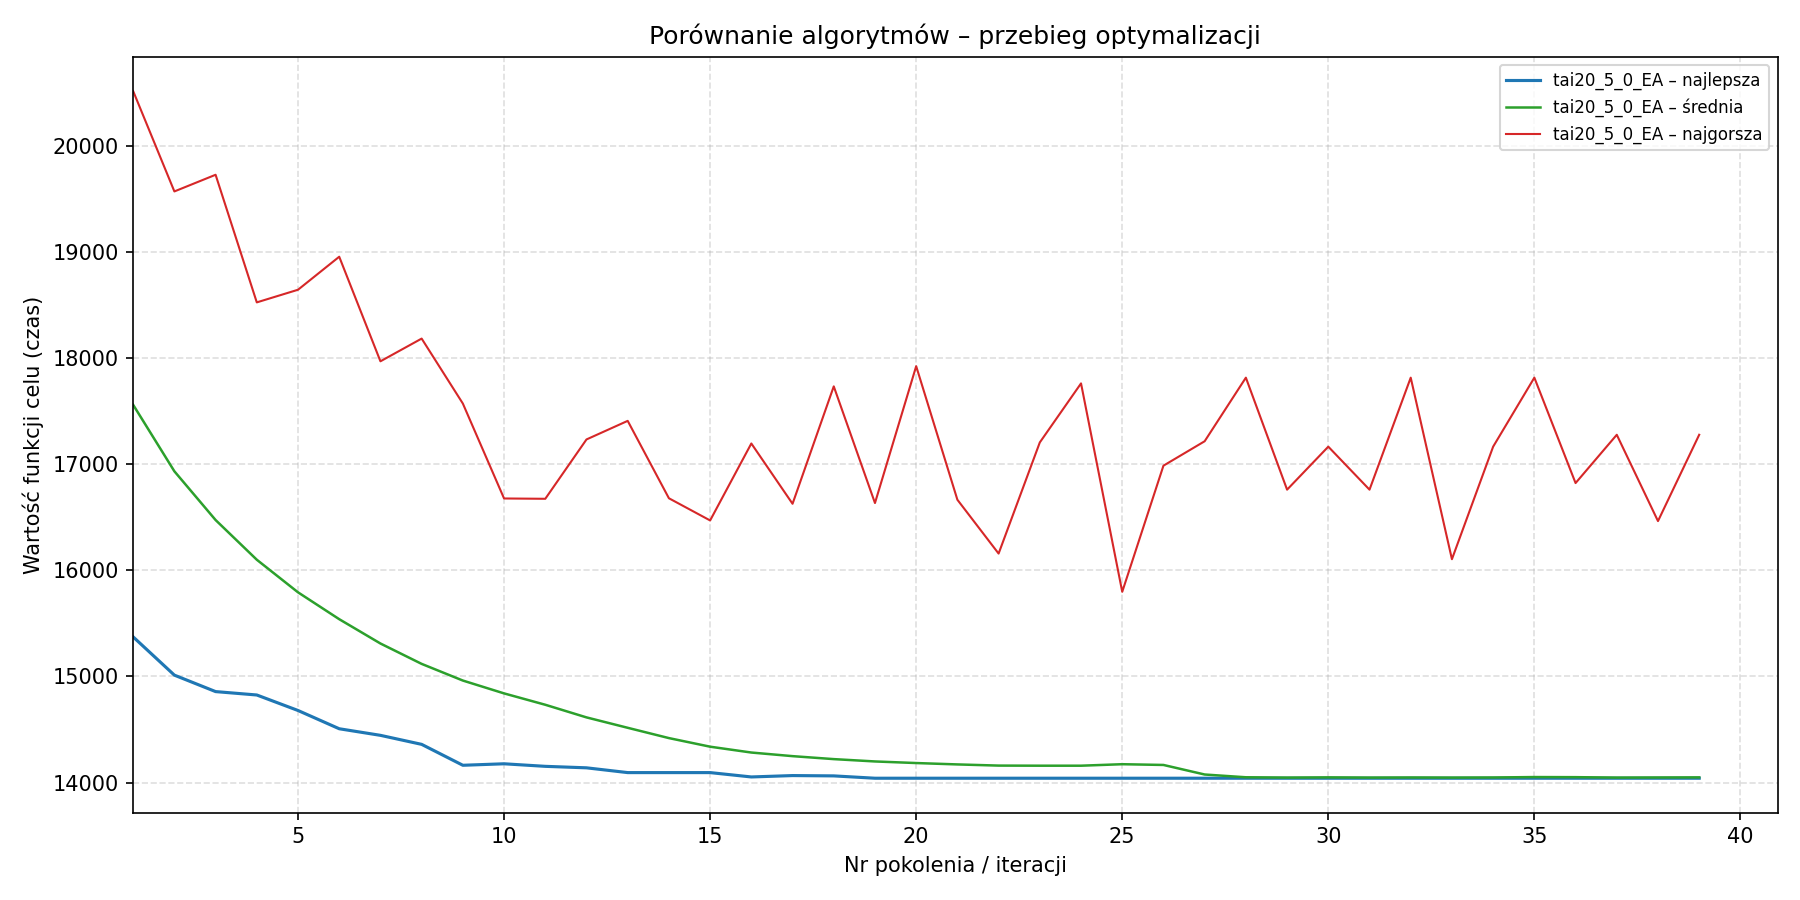
\includegraphics[width=0.9\textwidth]{tai20_5_0_EA.png}
    \caption{Przebieg EA dla instancji łatwej (tai20\_5, pop=5000, gen=39)}
\end{figure}

\begin{figure}[H]
    \centering
    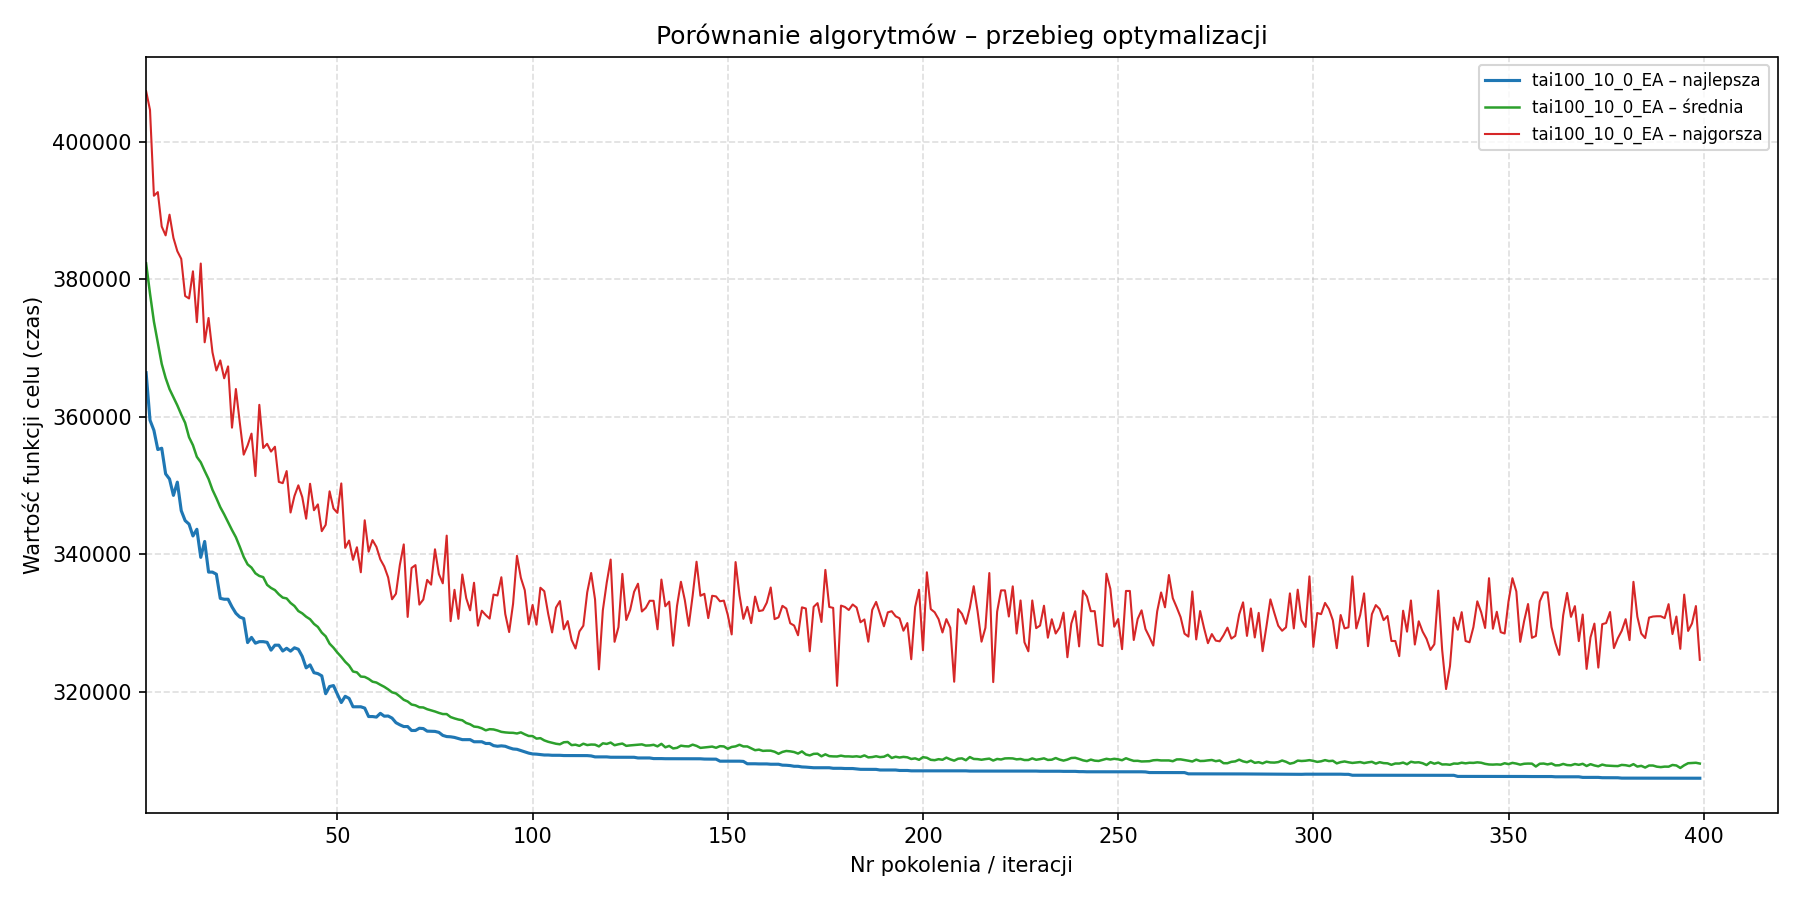
\includegraphics[width=0.9\textwidth]{tai100_10_0_EA.png}
    \caption{Przebieg EA dla instancji średniej (tai100\_10, pop=500, gen=399)}
\end{figure}

\begin{figure}[H]
    \centering
    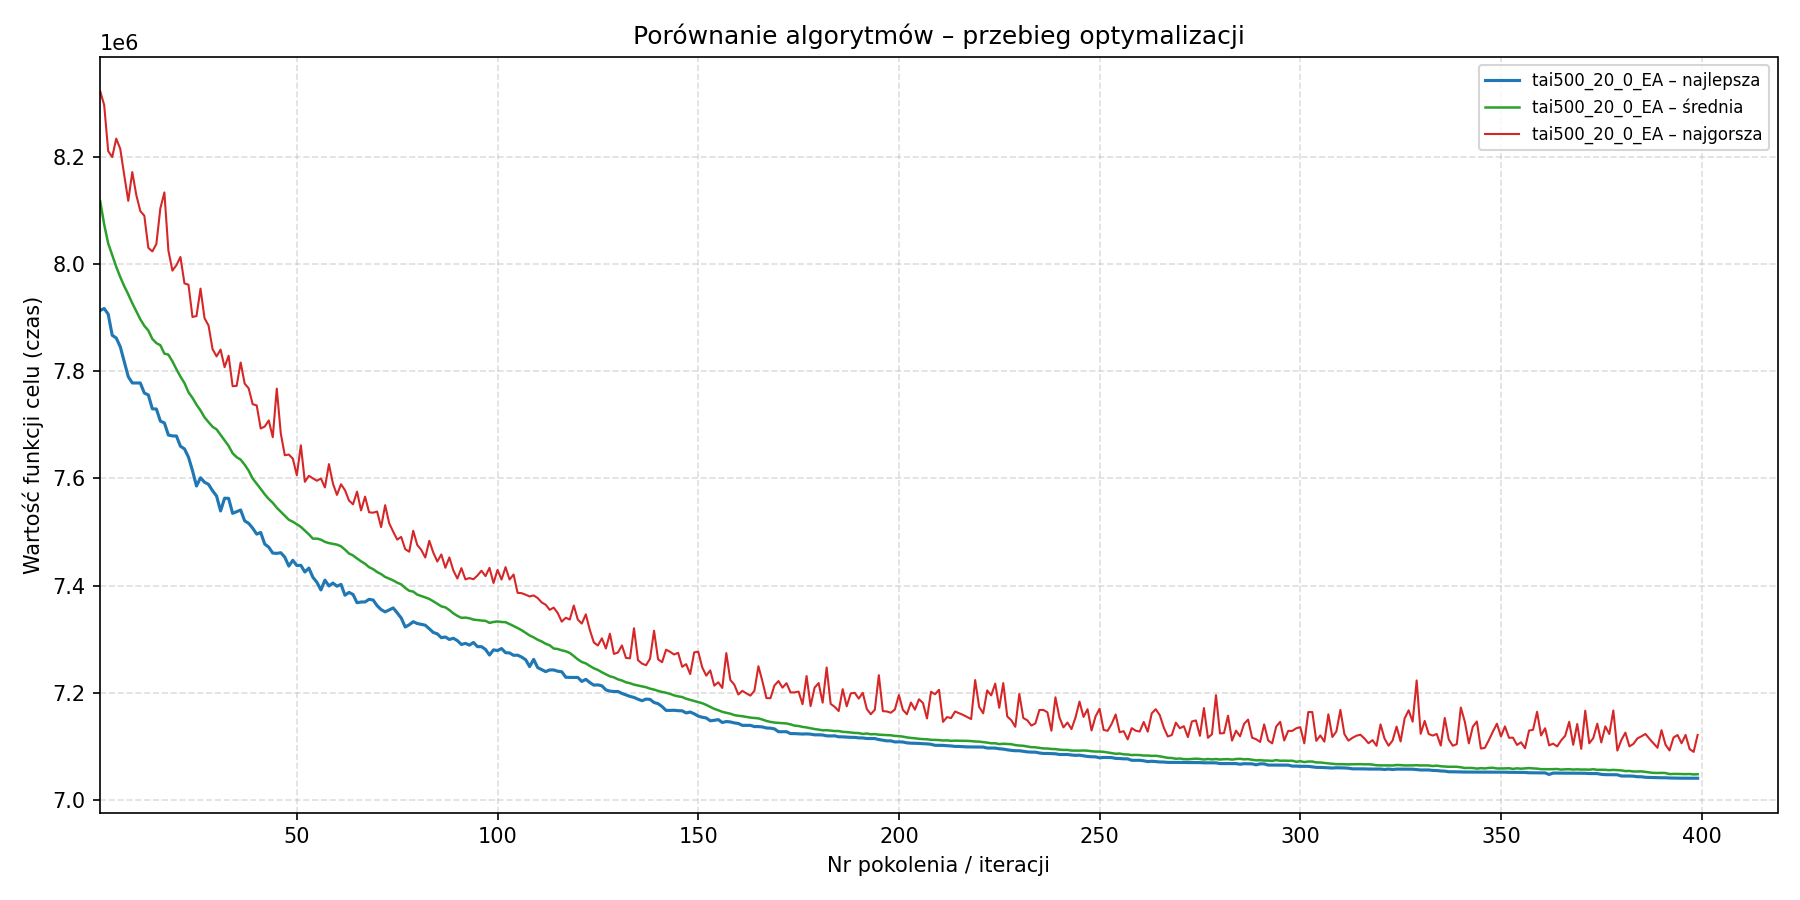
\includegraphics[width=0.9\textwidth]{tai500_20_0_EA.png}
    \caption{Przebieg EA dla instancji trudnej (tai500\_20, pop=500, gen=399)}
\end{figure}

\section{Analiza wyników i wnioski}
\label{sec:conclusions}

\subsection{Ranking algorytmów}

Na podstawie wyników finalnego porównania ustalono następujący ranking skuteczności:

\textbf{Instancje małe (tai20\_*):}
\begin{enumerate}
    \item \textbf{EA} -- wyraźnie najlepszy, z bardzo niskim odchyleniem standardowym (std=5.7--74.3). Duża populacja (5000) przy małej przestrzeni rozwiązań zapewniła doskonałe pokrycie i stabilność wyników.
    \item \textbf{SA} -- drugi, gorszy od EA o 1--2\%.
    \item \textbf{Random} -- trzeci, zbliżony do greedy.
    \item \textbf{Greedy} -- najgorszy na tai20\_10 i tai20\_20 (24611 vs EA 20911 -- różnica 17\%!). Greedy padał ofiarą minimów lokalnych już na etapie konstrukcji.
\end{enumerate}

\textbf{Instancje średnie i trudne (tai100\_*, tai500\_20):}
\begin{enumerate}
    \item \textbf{EA} -- nieznacznie lepszy od SA pod względem avg (tai100\_10: 309691 vs 311768, tai100\_20: 382019 vs 385475).
    \item \textbf{SA} -- zbliżony do EA.
    \item \textbf{Random} -- znacznie gorszy (tai100\_10: avg 357196 vs EA 309691, różnica 15\%).
    \item \textbf{Greedy} -- najgorszy (tai100\_10: 373462 vs EA 307448, różnica 21\%).
\end{enumerate}

\subsection{Kluczowe obserwacje}

\textbf{EA zdominowało SA na wszystkich dostępnych instancjach} po strojeniu -- stanowiło to odwrócenie wyniku sprzed strojenia, gdzie SA wygrywało na dużych instancjach. Strojenie parametrów EA (zwłaszcza per-instancja pop\_size, Px i Pm) miało decydujący wpływ na jakość wyników.

\textbf{Greedy okazało się najgorszą metodą} mimo że jest deterministyczne i szybkie. Jego budżet ewaluacji był znacznie mniejszy niż $B$ (np. 3820 ewaluacji dla tai20 vs 200k dla pozostałych), co utrudniało bezpośrednie porównanie. Nawet przy równym budżecie wyniki greedy nie dorównałyby metaheurystykom.

\textbf{Random okazało się zaskakująco dobrym} punktem odniesienia -- na instancjach tai20 osiągnęło wyniki zbliżone do greedy, a na tai100 było lepsze niż greedy. Wynikało to z bardzo dużej liczby ewaluacji ($B = 200\,000$) -- losowe próbkowanie przy takim budżecie pokrywało przestrzeń lepiej niż deterministyczna heurystyka z małą liczbą restartów.

\textbf{EA okazało się wyraźnie bardziej stabilne niż SA} -- odchylenie standardowe EA było konsekwentnie niższe (np. tai20\_5: std=5.7 EA vs 102.6 SA). Duża populacja i mechanizm elitaryzmu (zawsze zachowywane najlepsze rozwiązanie) zapewniały powtarzalność wyników.

\textbf{Strojenie per-instancja przyniosło znaczące korzyści.} Porównując wyniki bazowe EA (pop=100, avg tai100\_10=317724) z wynikami po strojeniu (pop=500, avg tai100\_10=309691) zaobserwowano poprawę o 2.5\%. Dla SA poprawa była mniejsza, co sugerowało że SA jest mniej wrażliwe na dobór parametrów przy odpowiednim budżecie obliczeniowym.

\end{document}
